\documentclass[twoside]{book}

% Packages required by doxygen
\usepackage{fixltx2e}
\usepackage{calc}
\usepackage{doxygen}
\usepackage[export]{adjustbox} % also loads graphicx
\usepackage{graphicx}
\usepackage[utf8]{inputenc}
\usepackage{makeidx}
\usepackage{multicol}
\usepackage{multirow}
\PassOptionsToPackage{warn}{textcomp}
\usepackage{textcomp}
\usepackage[nointegrals]{wasysym}
\usepackage[table]{xcolor}

% Font selection
\usepackage[T1]{fontenc}
\usepackage[scaled=.90]{helvet}
\usepackage{courier}
\usepackage{amssymb}
\usepackage{sectsty}
\renewcommand{\familydefault}{\sfdefault}
\allsectionsfont{%
  \fontseries{bc}\selectfont%
  \color{darkgray}%
}
\renewcommand{\DoxyLabelFont}{%
  \fontseries{bc}\selectfont%
  \color{darkgray}%
}
\newcommand{\+}{\discretionary{\mbox{\scriptsize$\hookleftarrow$}}{}{}}

% Page & text layout
\usepackage{geometry}
\geometry{%
  a4paper,%
  top=2.5cm,%
  bottom=2.5cm,%
  left=2.5cm,%
  right=2.5cm%
}
\tolerance=750
\hfuzz=15pt
\hbadness=750
\setlength{\emergencystretch}{15pt}
\setlength{\parindent}{0cm}
\setlength{\parskip}{3ex plus 2ex minus 2ex}
\makeatletter
\renewcommand{\paragraph}{%
  \@startsection{paragraph}{4}{0ex}{-1.0ex}{1.0ex}{%
    \normalfont\normalsize\bfseries\SS@parafont%
  }%
}
\renewcommand{\subparagraph}{%
  \@startsection{subparagraph}{5}{0ex}{-1.0ex}{1.0ex}{%
    \normalfont\normalsize\bfseries\SS@subparafont%
  }%
}
\makeatother

% Headers & footers
\usepackage{fancyhdr}
\pagestyle{fancyplain}
\fancyhead[LE]{\fancyplain{}{\bfseries\thepage}}
\fancyhead[CE]{\fancyplain{}{}}
\fancyhead[RE]{\fancyplain{}{\bfseries\leftmark}}
\fancyhead[LO]{\fancyplain{}{\bfseries\rightmark}}
\fancyhead[CO]{\fancyplain{}{}}
\fancyhead[RO]{\fancyplain{}{\bfseries\thepage}}
\fancyfoot[LE]{\fancyplain{}{}}
\fancyfoot[CE]{\fancyplain{}{}}
\fancyfoot[RE]{\fancyplain{}{\bfseries\scriptsize Generated by Doxygen }}
\fancyfoot[LO]{\fancyplain{}{\bfseries\scriptsize Generated by Doxygen }}
\fancyfoot[CO]{\fancyplain{}{}}
\fancyfoot[RO]{\fancyplain{}{}}
\renewcommand{\footrulewidth}{0.4pt}
\renewcommand{\chaptermark}[1]{%
  \markboth{#1}{}%
}
\renewcommand{\sectionmark}[1]{%
  \markright{\thesection\ #1}%
}

% Indices & bibliography
\usepackage{natbib}
\usepackage[titles]{tocloft}
\setcounter{tocdepth}{3}
\setcounter{secnumdepth}{5}
\makeindex

% Custom commands
\newcommand{\clearemptydoublepage}{%
  \newpage{\pagestyle{empty}\cleardoublepage}%
}

\usepackage{caption}
\captionsetup{labelsep=space,justification=centering,font={bf},singlelinecheck=off,skip=4pt,position=top}

%===== C O N T E N T S =====

\begin{document}

% Titlepage & ToC
\pagenumbering{alph}
\begin{titlepage}
\vspace*{7cm}
\begin{center}%
{\Large Big\+Integer for c++ }\\
\vspace*{1cm}
{\large Generated by Doxygen 1.8.13}\\
\end{center}
\end{titlepage}
\clearemptydoublepage
\pagenumbering{roman}
\tableofcontents
\clearemptydoublepage
\pagenumbering{arabic}

%--- Begin generated contents ---
\chapter{Big\+Integer\+C\+Plus\+Plus}
\label{md__r_e_a_d_m_e}
A Large Integer to help get past the the upper bound on the in-\/built largest integer available. 
\chapter{Class Index}
\section{Class List}
Here are the classes, structs, unions and interfaces with brief descriptions\+:\begin{DoxyCompactList}
\item\contentsline{section}{\textbf{ Add\+Result} \\*This class holds all of the methods for executing the long addition }{\pageref{struct_add_result}}{}
\item\contentsline{section}{\textbf{ Big\+Integer} }{\pageref{class_big_integer}}{}
\item\contentsline{section}{\textbf{ Big\+Int\+Utils} }{\pageref{class_big_int_utils}}{}
\item\contentsline{section}{\textbf{ Largest\+Array\+Result} \\*This class holds all of the utility methods used by the \doxyref{Big\+Integer}{p.}{class_big_integer} file }{\pageref{struct_largest_array_result}}{}
\item\contentsline{section}{\textbf{ Long\+Addition} }{\pageref{class_long_addition}}{}
\item\contentsline{section}{\textbf{ Long\+Subtraction} }{\pageref{class_long_subtraction}}{}
\item\contentsline{section}{\textbf{ Sub\+Result} \\*This class holds all of the methods for executing the long subtraction }{\pageref{struct_sub_result}}{}
\end{DoxyCompactList}

\chapter{File Index}
\section{File List}
Here is a list of all documented files with brief descriptions\+:\begin{DoxyCompactList}
\item\contentsline{section}{include/\textbf{ Big\+Integer.\+h} \\*This project is designed to add a larger integer type to C++ }{\pageref{_big_integer_8h}}{}
\item\contentsline{section}{include/{\bfseries Big\+Int\+Utils.\+h} }{\pageref{_big_int_utils_8h}}{}
\item\contentsline{section}{include/{\bfseries Long\+Addition.\+h} }{\pageref{_long_addition_8h}}{}
\end{DoxyCompactList}

\chapter{Class Documentation}
\section{Add\+Result Struct Reference}
\label{struct_add_result}\index{Add\+Result@{Add\+Result}}


This class holds all of the methods for executing the long addition.  




{\ttfamily \#include $<$Long\+Addition.\+h$>$}

\subsection*{Public Attributes}
\begin{DoxyCompactItemize}
\item 
int \textbf{ result}
\begin{DoxyCompactList}\small\item\em This value holds the single digit result from adding the two values. \end{DoxyCompactList}\item 
int \textbf{ carry\+Value}
\begin{DoxyCompactList}\small\item\em This value holds the remainder if applicable. \end{DoxyCompactList}\end{DoxyCompactItemize}


\subsection{Detailed Description}
This class holds all of the methods for executing the long addition. 

\subsection{D\+E\+S\+C\+R\+I\+P\+T\+I\+ON}\label{namespacestd_DESCRIPTION}
This class contains all of the methods neededfor checking and adding two integer values together. This class takes two integers provided by another class and runs a form of long division. This means that if the value ends up being two digits or increasing by greater than the value of 10, it adds 1 to the remainder value A struct. This struct is used for storing the result returned by adding the first and second value and also the remainder. 

\subsection{Member Data Documentation}
\mbox{\label{struct_add_result_a06d99d9daaebd0528d158e86441fd189}} 
\index{Add\+Result@{Add\+Result}!carry\+Value@{carry\+Value}}
\index{carry\+Value@{carry\+Value}!Add\+Result@{Add\+Result}}
\subsubsection{carry\+Value}
{\footnotesize\ttfamily int Add\+Result\+::carry\+Value}



This value holds the remainder if applicable. 

\mbox{\label{struct_add_result_ae66aa315e5c177a4d85abe034b59cc58}} 
\index{Add\+Result@{Add\+Result}!result@{result}}
\index{result@{result}!Add\+Result@{Add\+Result}}
\subsubsection{result}
{\footnotesize\ttfamily int Add\+Result\+::result}



This value holds the single digit result from adding the two values. 



The documentation for this struct was generated from the following file\+:\begin{DoxyCompactItemize}
\item 
include/Long\+Addition.\+h\end{DoxyCompactItemize}

\section{Add\+Two\+Values\+Result Struct Reference}
\label{struct_add_two_values_result}\index{Add\+Two\+Values\+Result@{Add\+Two\+Values\+Result}}
\subsection*{Public Attributes}
\begin{DoxyCompactItemize}
\item 
\mbox{\label{struct_add_two_values_result_ad5f173a76df5cfda233ac1e04701062c}} 
int $\ast$ {\bfseries array}
\end{DoxyCompactItemize}


The documentation for this struct was generated from the following file\+:\begin{DoxyCompactItemize}
\item 
include/Big\+Int\+Utils.\+h\end{DoxyCompactItemize}

\section{Big\+Integer Class Reference}
\label{class_big_integer}\index{Big\+Integer@{Big\+Integer}}
\subsection*{Public Member Functions}
\begin{DoxyCompactItemize}
\item 
\textbf{ Big\+Integer} ()
\begin{DoxyCompactList}\small\item\em A constructor. \end{DoxyCompactList}\item 
\textbf{ $\sim$\+Big\+Integer} ()
\begin{DoxyCompactList}\small\item\em A destructor. \end{DoxyCompactList}\item 
void \textbf{ set\+Value} (string int\+Value)
\begin{DoxyCompactList}\small\item\em Sets the value of the \doxyref{Big\+Integer}{p.}{class_big_integer} variable. \end{DoxyCompactList}\item 
void \textbf{ set\+Value} (long long int big\+Int\+Value)
\begin{DoxyCompactList}\small\item\em Sets the value of the \doxyref{Big\+Integer}{p.}{class_big_integer} variable. \end{DoxyCompactList}\item 
unsigned long \textbf{ get\+Length} ()
\begin{DoxyCompactList}\small\item\em Retrieves the length of the number held by the variable. \end{DoxyCompactList}\item 
int $\ast$ \textbf{ get\+Value} ()
\begin{DoxyCompactList}\small\item\em This method is used to retrieve the current value stored in the \doxyref{Big\+Integer}{p.}{class_big_integer} variable. \end{DoxyCompactList}\item 
void \textbf{ print\+Value} ()
\begin{DoxyCompactList}\small\item\em This method is used for printing thr value of the \doxyref{Big\+Integer}{p.}{class_big_integer} value. \end{DoxyCompactList}\item 
void \textbf{ add} (\textbf{ Big\+Integer} first\+Val, \textbf{ Big\+Integer} second\+Val)
\begin{DoxyCompactList}\small\item\em This method is used to add two \doxyref{Big\+Integer}{p.}{class_big_integer} values. \end{DoxyCompactList}\item 
void \textbf{ subtract} (\textbf{ Big\+Integer} first\+Val, \textbf{ Big\+Integer} second\+Val)
\begin{DoxyCompactList}\small\item\em This method is used to subtract one \doxyref{Big\+Integer}{p.}{class_big_integer} value from another. \end{DoxyCompactList}\item 
void \textbf{ multiply} (\textbf{ Big\+Integer} first\+Val, \textbf{ Big\+Integer} second\+Val)
\begin{DoxyCompactList}\small\item\em This method is used to multiply two \doxyref{Big\+Integer}{p.}{class_big_integer} values together. \end{DoxyCompactList}\item 
void \textbf{ divide} (\textbf{ Big\+Integer} first\+Val, \textbf{ Big\+Integer} second\+Val)
\begin{DoxyCompactList}\small\item\em This method is used to divide two \doxyref{Big\+Integer}{p.}{class_big_integer} values together. \end{DoxyCompactList}\end{DoxyCompactItemize}


\subsection{Constructor \& Destructor Documentation}
\mbox{\label{class_big_integer_a67a108dbe651911a21b3fc4310a505dd}} 
\index{Big\+Integer@{Big\+Integer}!Big\+Integer@{Big\+Integer}}
\index{Big\+Integer@{Big\+Integer}!Big\+Integer@{Big\+Integer}}
\subsubsection{Big\+Integer()}
{\footnotesize\ttfamily Big\+Integer\+::\+Big\+Integer (\begin{DoxyParamCaption}\item[{void}]{ }\end{DoxyParamCaption})}



A constructor. 

Constructor for creating a \doxyref{Big\+Integer}{p.}{class_big_integer}. \mbox{\label{class_big_integer_a987e3a4e9c4405404719be08caaa3146}} 
\index{Big\+Integer@{Big\+Integer}!````~Big\+Integer@{$\sim$\+Big\+Integer}}
\index{````~Big\+Integer@{$\sim$\+Big\+Integer}!Big\+Integer@{Big\+Integer}}
\subsubsection{$\sim$\+Big\+Integer()}
{\footnotesize\ttfamily Big\+Integer\+::$\sim$\+Big\+Integer (\begin{DoxyParamCaption}\item[{void}]{ }\end{DoxyParamCaption})}



A destructor. 

Removes the constructor when the program ends. 

\subsection{Member Function Documentation}
\mbox{\label{class_big_integer_a02fe8d89a8d0f5796d77e852ea49e8ae}} 
\index{Big\+Integer@{Big\+Integer}!add@{add}}
\index{add@{add}!Big\+Integer@{Big\+Integer}}
\subsubsection{add()}
{\footnotesize\ttfamily void Big\+Integer\+::add (\begin{DoxyParamCaption}\item[{\textbf{ Big\+Integer}}]{first\+Val,  }\item[{\textbf{ Big\+Integer}}]{second\+Val }\end{DoxyParamCaption})}



This method is used to add two \doxyref{Big\+Integer}{p.}{class_big_integer} values. 


\begin{DoxyParams}{Parameters}
{\em first\+Val} & is the first \doxyref{Big\+Integer}{p.}{class_big_integer} value to be added. \\
\hline
{\em second\+Val} & is the second \doxyref{Big\+Integer}{p.}{class_big_integer} value to be added. \\
\hline
\end{DoxyParams}
\begin{DoxySeeAlso}{See also}
\doxyref{Big\+Integer()}{p.}{class_big_integer_a67a108dbe651911a21b3fc4310a505dd} 

\doxyref{$\sim$\+Big\+Integer()}{p.}{class_big_integer_a987e3a4e9c4405404719be08caaa3146} 

\doxyref{set\+Value(string int\+Value)}{p.}{class_big_integer_aaf261f212247b3206108902c039a8133} 

\doxyref{set\+Value(long long int big\+Int\+Value)}{p.}{class_big_integer_a8dbfc69090df350ac479814694f46ca8}
\end{DoxySeeAlso}
The result is then assigned to the \doxyref{Big\+Integer}{p.}{class_big_integer} value it is appended to. It adds the two values using a form of long division adding individual digits one at a time, starting from the end of both arrays, and carrying over a 1 if the result exceeds 10. It then stores this in a new array to be stored in a \doxyref{Big\+Integer}{p.}{class_big_integer} variable.

Example of use\+: 
\begin{DoxyCode}
BigInteger firstVal.setValue(\textcolor{stringliteral}{"20"}); \textcolor{comment}{// Create variable and assign it the value 20.}
BigInteger secondValue.setValue(\textcolor{stringliteral}{"15"}); \textcolor{comment}{// Create variable and assign it the value 15.}

BigInteger result.add(firstVal,secondValue); \textcolor{comment}{// Add both values and append the answer, 35, the BigInteger
       result.}
\end{DoxyCode}
 \mbox{\label{class_big_integer_afb86ffe260608c44af94e430a2ee4b82}} 
\index{Big\+Integer@{Big\+Integer}!divide@{divide}}
\index{divide@{divide}!Big\+Integer@{Big\+Integer}}
\subsubsection{divide()}
{\footnotesize\ttfamily void Big\+Integer\+::divide (\begin{DoxyParamCaption}\item[{\textbf{ Big\+Integer}}]{first\+Val,  }\item[{\textbf{ Big\+Integer}}]{second\+Val }\end{DoxyParamCaption})}



This method is used to divide two \doxyref{Big\+Integer}{p.}{class_big_integer} values together. 


\begin{DoxyParams}{Parameters}
{\em first\+Val} & is the first value to multiply. \\
\hline
{\em second\+Val} & is the second value to multiply. \\
\hline
\end{DoxyParams}
\begin{DoxySeeAlso}{See also}


\doxyref{Big\+Integer()}{p.}{class_big_integer_a67a108dbe651911a21b3fc4310a505dd} 

\doxyref{$\sim$\+Big\+Integer()}{p.}{class_big_integer_a987e3a4e9c4405404719be08caaa3146} 

\doxyref{set\+Value(string int\+Value)}{p.}{class_big_integer_aaf261f212247b3206108902c039a8133} 

\doxyref{set\+Value(long long int big\+Int\+Value)}{p.}{class_big_integer_a8dbfc69090df350ac479814694f46ca8}
\end{DoxySeeAlso}
This method is used to divide the first \doxyref{Big\+Integer}{p.}{class_big_integer} number by the second \doxyref{Big\+Integer}{p.}{class_big_integer} number.

Example of use\+: 
\begin{DoxyCode}
BigInteger firstNumber.setValue(30); \textcolor{comment}{// Assign the number 30 to the variable firstNumber.}
BigInteger secondNumber.setValue(6); \textcolor{comment}{// Assign the number 6 to the variable secondNumber.}

BigInteger result.divide(firstNumber,secondNumber); \textcolor{comment}{// Assigns the result of dividing the firstNumber by
       the secondNumber.}
\end{DoxyCode}
 \mbox{\label{class_big_integer_ab1f0e41f6cba177600f6965f4a0b5329}} 
\index{Big\+Integer@{Big\+Integer}!get\+Length@{get\+Length}}
\index{get\+Length@{get\+Length}!Big\+Integer@{Big\+Integer}}
\subsubsection{get\+Length()}
{\footnotesize\ttfamily unsigned long Big\+Integer\+::get\+Length (\begin{DoxyParamCaption}{ }\end{DoxyParamCaption})}



Retrieves the length of the number held by the variable. 

\begin{DoxyReturn}{Returns}
The length of the number. 
\end{DoxyReturn}
\begin{DoxySeeAlso}{See also}
\doxyref{Big\+Integer()}{p.}{class_big_integer_a67a108dbe651911a21b3fc4310a505dd} 

\doxyref{$\sim$\+Big\+Integer()}{p.}{class_big_integer_a987e3a4e9c4405404719be08caaa3146} 

\doxyref{set\+Value(string int\+Value)}{p.}{class_big_integer_aaf261f212247b3206108902c039a8133}
\end{DoxySeeAlso}
This method is used for retrieving the length of the number in the \doxyref{Big\+Integer}{p.}{class_big_integer} variable. This method is mainly used by other methods, however, was kept public so the user can use and access it.

Example of use\+: 
\begin{DoxyCode}
BigInteger test.getLength(); \textcolor{comment}{// Will return the length of the array stored in the variable test.}
\end{DoxyCode}
 \mbox{\label{class_big_integer_adcf3fa048a5fe4c9828475e1eace1031}} 
\index{Big\+Integer@{Big\+Integer}!get\+Value@{get\+Value}}
\index{get\+Value@{get\+Value}!Big\+Integer@{Big\+Integer}}
\subsubsection{get\+Value()}
{\footnotesize\ttfamily int $\ast$ Big\+Integer\+::get\+Value (\begin{DoxyParamCaption}{ }\end{DoxyParamCaption})}



This method is used to retrieve the current value stored in the \doxyref{Big\+Integer}{p.}{class_big_integer} variable. 

\begin{DoxyReturn}{Returns}
The pointer to the start of the array containing the number.
\end{DoxyReturn}
The numbers stored in the \doxyref{Big\+Integer}{p.}{class_big_integer} type are stored as an array. This means in order to access their results we access them by using a pointer to the start of the array.

Example of use\+: 
\begin{DoxyCode}
BigInteger test.getValue(); \textcolor{comment}{// Returns a pointer to the start of the array holding the value of the
       BigInteger variable test.}
\end{DoxyCode}
 \mbox{\label{class_big_integer_a29ed82a225776f7b2237789fbd7c1cf9}} 
\index{Big\+Integer@{Big\+Integer}!multiply@{multiply}}
\index{multiply@{multiply}!Big\+Integer@{Big\+Integer}}
\subsubsection{multiply()}
{\footnotesize\ttfamily void Big\+Integer\+::multiply (\begin{DoxyParamCaption}\item[{\textbf{ Big\+Integer}}]{first\+Val,  }\item[{\textbf{ Big\+Integer}}]{second\+Val }\end{DoxyParamCaption})}



This method is used to multiply two \doxyref{Big\+Integer}{p.}{class_big_integer} values together. 


\begin{DoxyParams}{Parameters}
{\em first\+Val} & is the first value to multiply. \\
\hline
{\em second\+Val} & is the second value to multiply. \\
\hline
\end{DoxyParams}
\begin{DoxySeeAlso}{See also}


\doxyref{Big\+Integer()}{p.}{class_big_integer_a67a108dbe651911a21b3fc4310a505dd} 

\doxyref{$\sim$\+Big\+Integer()}{p.}{class_big_integer_a987e3a4e9c4405404719be08caaa3146} 

\doxyref{set\+Value(string int\+Value)}{p.}{class_big_integer_aaf261f212247b3206108902c039a8133} 

\doxyref{set\+Value(long long int big\+Int\+Value)}{p.}{class_big_integer_a8dbfc69090df350ac479814694f46ca8}
\end{DoxySeeAlso}
This method is used to multiply two \doxyref{Big\+Integer}{p.}{class_big_integer} numbers together.

Example of use\+: 
\begin{DoxyCode}
BigInteger firstNumber.setValue(20); \textcolor{comment}{// Assign the number 20 to the variable firstNumber.}
BigInteger secondNumber.setValue(55); \textcolor{comment}{// Assign the number 55 to the variable secondNumber.}

BigInteger result.multiply(firstNumber,secondNumber); \textcolor{comment}{// Assigns the result of multiplying the firstNumber
       and the secondNumber.}
\end{DoxyCode}
 \mbox{\label{class_big_integer_a97b276cd2141c659e76843e93ce85429}} 
\index{Big\+Integer@{Big\+Integer}!print\+Value@{print\+Value}}
\index{print\+Value@{print\+Value}!Big\+Integer@{Big\+Integer}}
\subsubsection{print\+Value()}
{\footnotesize\ttfamily void Big\+Integer\+::print\+Value (\begin{DoxyParamCaption}{ }\end{DoxyParamCaption})}



This method is used for printing thr value of the \doxyref{Big\+Integer}{p.}{class_big_integer} value. 

As the values are stored as arrays, this method iterates through, printing each number in sequence.

example of use\+: 
\begin{DoxyCode}
BigInteger test.printValue(); \textcolor{comment}{// Prints the value of test correctly.}
\end{DoxyCode}
 \mbox{\label{class_big_integer_aaf261f212247b3206108902c039a8133}} 
\index{Big\+Integer@{Big\+Integer}!set\+Value@{set\+Value}}
\index{set\+Value@{set\+Value}!Big\+Integer@{Big\+Integer}}
\subsubsection{set\+Value()\hspace{0.1cm}{\footnotesize\ttfamily [1/2]}}
{\footnotesize\ttfamily void Big\+Integer\+::set\+Value (\begin{DoxyParamCaption}\item[{string}]{int\+Value }\end{DoxyParamCaption})}



Sets the value of the \doxyref{Big\+Integer}{p.}{class_big_integer} variable. 


\begin{DoxyParams}{Parameters}
{\em int\+Value} & is the String representation of the number the user wants to be stored in the \doxyref{Big\+Integer}{p.}{class_big_integer} variable. \\
\hline
\end{DoxyParams}
\begin{DoxySeeAlso}{See also}
\doxyref{Big\+Integer()}{p.}{class_big_integer_a67a108dbe651911a21b3fc4310a505dd} 

\doxyref{$\sim$\+Big\+Integer()}{p.}{class_big_integer_a987e3a4e9c4405404719be08caaa3146} 

\doxyref{get\+Value()}{p.}{class_big_integer_adcf3fa048a5fe4c9828475e1eace1031} 

\doxyref{print\+Value()}{p.}{class_big_integer_a97b276cd2141c659e76843e93ce85429}
\end{DoxySeeAlso}
This sets the current \doxyref{Big\+Integer}{p.}{class_big_integer} variable to be the numerical Type of the String number entered by the user. Although this method does not return any values it does assign the value to a the \doxyref{Big\+Integer}{p.}{class_big_integer} value when appended.

Example of use\+: 
\begin{DoxyCode}
BigInteger test.setValue(\textcolor{stringliteral}{"143654543242"}); \textcolor{comment}{// Assigns the string 143654543242 to the variable test}
\end{DoxyCode}
 \mbox{\label{class_big_integer_a8dbfc69090df350ac479814694f46ca8}} 
\index{Big\+Integer@{Big\+Integer}!set\+Value@{set\+Value}}
\index{set\+Value@{set\+Value}!Big\+Integer@{Big\+Integer}}
\subsubsection{set\+Value()\hspace{0.1cm}{\footnotesize\ttfamily [2/2]}}
{\footnotesize\ttfamily void Big\+Integer\+::set\+Value (\begin{DoxyParamCaption}\item[{long long int}]{big\+Int\+Value }\end{DoxyParamCaption})}



Sets the value of the \doxyref{Big\+Integer}{p.}{class_big_integer} variable. 


\begin{DoxyParams}{Parameters}
{\em big\+Int\+Value} & is the long long int representation of the number the user wants to be stored in the \doxyref{Big\+Integer}{p.}{class_big_integer} variable. \\
\hline
\end{DoxyParams}
\begin{DoxySeeAlso}{See also}
\doxyref{Big\+Integer()}{p.}{class_big_integer_a67a108dbe651911a21b3fc4310a505dd} 

\doxyref{$\sim$\+Big\+Integer()}{p.}{class_big_integer_a987e3a4e9c4405404719be08caaa3146} 

\doxyref{set\+Value(long long int big\+Int\+Value)}{p.}{class_big_integer_a8dbfc69090df350ac479814694f46ca8} 

\doxyref{get\+Value()}{p.}{class_big_integer_adcf3fa048a5fe4c9828475e1eace1031} 

\doxyref{print\+Value()}{p.}{class_big_integer_a97b276cd2141c659e76843e93ce85429}
\end{DoxySeeAlso}
Similar to the method \doxyref{set\+Value(string int\+Value)}{p.}{class_big_integer_aaf261f212247b3206108902c039a8133} this allows for the use of the method with a long long int argument. This is a form of method overloading allowing for both methods to be viable and also providing the use of the function with an argument of differing types.

Example of use\+: 
\begin{DoxyCode}
BigInteger test.setValue(54234243); \textcolor{comment}{// Assigns the number 54234243 to the variable test}
\end{DoxyCode}
 \mbox{\label{class_big_integer_a7725b32ee3492ffd2c263ae53c2c9126}} 
\index{Big\+Integer@{Big\+Integer}!subtract@{subtract}}
\index{subtract@{subtract}!Big\+Integer@{Big\+Integer}}
\subsubsection{subtract()}
{\footnotesize\ttfamily void Big\+Integer\+::subtract (\begin{DoxyParamCaption}\item[{\textbf{ Big\+Integer}}]{first\+Val,  }\item[{\textbf{ Big\+Integer}}]{second\+Val }\end{DoxyParamCaption})}



This method is used to subtract one \doxyref{Big\+Integer}{p.}{class_big_integer} value from another. 


\begin{DoxyParams}{Parameters}
{\em first\+Val} & is the number to have a value subtracted from. \\
\hline
{\em second\+Val} & is the number to subtract. \\
\hline
\end{DoxyParams}
\begin{DoxyReturn}{Returns}
the result of subtracting second\+Val from first\+Val. 
\end{DoxyReturn}
\begin{DoxySeeAlso}{See also}


\doxyref{Big\+Integer()}{p.}{class_big_integer_a67a108dbe651911a21b3fc4310a505dd} 

\doxyref{$\sim$\+Big\+Integer()}{p.}{class_big_integer_a987e3a4e9c4405404719be08caaa3146} 

\doxyref{set\+Value(string int\+Value)}{p.}{class_big_integer_aaf261f212247b3206108902c039a8133} 

\doxyref{set\+Value(long long int big\+Int\+Value)}{p.}{class_big_integer_a8dbfc69090df350ac479814694f46ca8}
\end{DoxySeeAlso}
This method is used for subtracting one value from another. It takes a similar approach to add using a form of long subtraction. It odes the calculations one digit at a time and carries over any number that exeeds two digits.

Example of use\+: 
\begin{DoxyCode}
BigInteger firstNumber.setValue(\textcolor{stringliteral}{"100"}); \textcolor{comment}{// Assign the number 100 to the variable firstNumber.}
BigInteger secondNumber.setValue(\textcolor{stringliteral}{"20"}); \textcolor{comment}{// Assign the number 20 to the variable secondNumber.}

BigInteger result.subtract(firstNumber,secondNumber); \textcolor{comment}{// Assigns the result of subtracting secondNumber
       from firstNumber, giving the result 80, to the variable result.}
\end{DoxyCode}
 

The documentation for this class was generated from the following files\+:\begin{DoxyCompactItemize}
\item 
include/Big\+Integer.\+h\item 
src/\+Big\+Int\+Components/Big\+Integer.\+cpp\end{DoxyCompactItemize}

\section{Big\+Int\+Utils Class Reference}
\label{class_big_int_utils}\index{Big\+Int\+Utils@{Big\+Int\+Utils}}
\subsection*{Public Member Functions}
\begin{DoxyCompactItemize}
\item 
\textbf{ Largest\+Array\+Result} \textbf{ get\+Largest\+Array} (\textbf{ Big\+Integer} first\+Val, \textbf{ Big\+Integer} second\+Val)
\begin{DoxyCompactList}\small\item\em This method is used for getting the larger of the two arrays and returning the values discussed in the struct \doxyref{Largest\+Array\+Result}{p.}{struct_largest_array_result}. \end{DoxyCompactList}\item 
int $\ast$ \textbf{ add\+Two\+Values} (int $\ast$first\+Num, int $\ast$second\+Num, \textbf{ Largest\+Array\+Result} result)
\begin{DoxyCompactList}\small\item\em This method is used to correctly add two \doxyref{Big\+Integer}{p.}{class_big_integer} values. \end{DoxyCompactList}\item 
int $\ast$ \textbf{ sub\+Two\+Values} (int $\ast$first\+Num, int $\ast$second\+Num, \textbf{ Largest\+Array\+Result} result)
\begin{DoxyCompactList}\small\item\em [sub\+Two\+Values description]  sub\+Two\+Values \end{DoxyCompactList}\end{DoxyCompactItemize}


\subsection{Member Function Documentation}
\mbox{\label{class_big_int_utils_a593ae84f25f4472e9dba017969dc2d24}} 
\index{Big\+Int\+Utils@{Big\+Int\+Utils}!add\+Two\+Values@{add\+Two\+Values}}
\index{add\+Two\+Values@{add\+Two\+Values}!Big\+Int\+Utils@{Big\+Int\+Utils}}
\subsubsection{add\+Two\+Values()}
{\footnotesize\ttfamily int $\ast$ Big\+Int\+Utils\+::add\+Two\+Values (\begin{DoxyParamCaption}\item[{int $\ast$}]{first\+Num,  }\item[{int $\ast$}]{second\+Num,  }\item[{\textbf{ Largest\+Array\+Result}}]{result }\end{DoxyParamCaption})}



This method is used to correctly add two \doxyref{Big\+Integer}{p.}{class_big_integer} values. 


\begin{DoxyParams}{Parameters}
{\em first\+Num} & is the first \doxyref{Big\+Integer}{p.}{class_big_integer} variable to be added. \\
\hline
{\em second\+Num} & is the second \doxyref{Big\+Integer}{p.}{class_big_integer} variable to be added. \\
\hline
{\em result} & is the variable storing the lengths of the array as well as the difference in size and which of the two arrays is larger. \\
\hline
\end{DoxyParams}
\begin{DoxyReturn}{Returns}
is the answer to be stored in a \doxyref{Big\+Integer}{p.}{class_big_integer} result variable. 
\end{DoxyReturn}
\begin{DoxySeeAlso}{See also}
\doxyref{Largest\+Array\+Result}{p.}{struct_largest_array_result} 

\doxyref{get\+Largest\+Array(\+Big\+Integer first\+Val, Big\+Integer second\+Val)}{p.}{class_big_int_utils_a6f355ec25a51cf1f480966d6d0780ea4}
\end{DoxySeeAlso}
This method is used to iterate through all of the values in both arrays and add them. It starts from the end of both arrays and adds them a digit at a time. It then carries over any additional value and adds that to the next addition. It does this until there are no more numbers to add and returns this value. This mthod is used by the Program and isn\textquotesingle{}t used by the user. \mbox{\label{class_big_int_utils_a6f355ec25a51cf1f480966d6d0780ea4}} 
\index{Big\+Int\+Utils@{Big\+Int\+Utils}!get\+Largest\+Array@{get\+Largest\+Array}}
\index{get\+Largest\+Array@{get\+Largest\+Array}!Big\+Int\+Utils@{Big\+Int\+Utils}}
\subsubsection{get\+Largest\+Array()}
{\footnotesize\ttfamily \textbf{ Largest\+Array\+Result} Big\+Int\+Utils\+::get\+Largest\+Array (\begin{DoxyParamCaption}\item[{\textbf{ Big\+Integer}}]{first\+Val,  }\item[{\textbf{ Big\+Integer}}]{second\+Val }\end{DoxyParamCaption})}



This method is used for getting the larger of the two arrays and returning the values discussed in the struct \doxyref{Largest\+Array\+Result}{p.}{struct_largest_array_result}. 

get\+Largest\+Array 
\begin{DoxyParams}{Parameters}
{\em first\+Val} & is the first array. \\
\hline
{\em second\+Val} & is the second array. \\
\hline
\end{DoxyParams}
\begin{DoxyReturn}{Returns}
a struct containing the length of the largest and smallest array, the difference as well as a boolean value saying which array is longer. 
\end{DoxyReturn}
\begin{DoxySeeAlso}{See also}
\doxyref{Largest\+Array\+Result}{p.}{struct_largest_array_result}
\end{DoxySeeAlso}
This method is used for getting the length of the largest array ad returning it. It also makes a not of the length of the other array as well as the difference. This data is used for when using any of the operator fuctions as they make use of the array length. Having both lengths is neccessary as both arrays may be different lengths. Having the boolean value also helps to distinguish which array is longer too.

Example of use\+: 
\begin{DoxyCode}
BigInteger arrayOne.setValue(23434324); \textcolor{comment}{// Sets the value of the first BigInteger variable to 23434324.}
BigInteger arrayTwo.setValue(2434); \textcolor{comment}{// Sets the value of the second BigInteger variable to 2434.}

LargestArrayResult result = getLargestArray(arrayTwo,arrayTwo); \textcolor{comment}{// Returns the length of the arrays and
       which of the arrays is larger.}
\end{DoxyCode}
 \mbox{\label{class_big_int_utils_a03e7832da59466f499da43cf84378510}} 
\index{Big\+Int\+Utils@{Big\+Int\+Utils}!sub\+Two\+Values@{sub\+Two\+Values}}
\index{sub\+Two\+Values@{sub\+Two\+Values}!Big\+Int\+Utils@{Big\+Int\+Utils}}
\subsubsection{sub\+Two\+Values()}
{\footnotesize\ttfamily int$\ast$ Big\+Int\+Utils\+::sub\+Two\+Values (\begin{DoxyParamCaption}\item[{int $\ast$}]{first\+Num,  }\item[{int $\ast$}]{second\+Num,  }\item[{\textbf{ Largest\+Array\+Result}}]{result }\end{DoxyParamCaption})}



[sub\+Two\+Values description]  sub\+Two\+Values 


\begin{DoxyParams}{Parameters}
{\em first\+Num} & \\
\hline
{\em second\+Num} & \\
\hline
{\em result} & \\
\hline
\end{DoxyParams}
\begin{DoxyReturn}{Returns}

\end{DoxyReturn}
Example of use\+: 
\begin{DoxyCode}
\end{DoxyCode}
 

The documentation for this class was generated from the following files\+:\begin{DoxyCompactItemize}
\item 
include/Big\+Int\+Utils.\+h\item 
src/\+Big\+Int\+Components/Big\+Int\+Utils.\+cpp\end{DoxyCompactItemize}

\section{Largest\+Array\+Result Struct Reference}
\label{struct_largest_array_result}\index{Largest\+Array\+Result@{Largest\+Array\+Result}}


This class holds all of the utility methods used by the \doxyref{Big\+Integer}{p.}{class_big_integer} file.  




{\ttfamily \#include $<$Big\+Int\+Utils.\+h$>$}

\subsection*{Public Attributes}
\begin{DoxyCompactItemize}
\item 
unsigned long \textbf{ big}
\begin{DoxyCompactList}\small\item\em The length of the largest array. \end{DoxyCompactList}\item 
unsigned long \textbf{ small}
\begin{DoxyCompactList}\small\item\em The length of the smallest array. \end{DoxyCompactList}\item 
unsigned long \textbf{ diff}
\begin{DoxyCompactList}\small\item\em The length of the difference between the sizes of the two arrays. \end{DoxyCompactList}\item 
bool \textbf{ is\+First\+Val\+Bigger}
\begin{DoxyCompactList}\small\item\em The boolean value for saying which of the two arrays is largest. \end{DoxyCompactList}\end{DoxyCompactItemize}


\subsection{Detailed Description}
This class holds all of the utility methods used by the \doxyref{Big\+Integer}{p.}{class_big_integer} file. 

\subsection{D\+E\+S\+C\+R\+I\+P\+T\+I\+ON}\label{namespacestd_DESCRIPTION}
This file contains all of the utility methods for use by \doxyref{Big\+Integer}{p.}{class_big_integer}. This helps to spread out the program and prevent all of the code sitting in one file bulking it and making it harder to edit or debug. A struct. This is used for storing the vlaues of which array is the longest and the difference between two arrays. It also has a boolean value for saying which of the two arrays is longer. 

\subsection{Member Data Documentation}
\mbox{\label{struct_largest_array_result_a52ebc79f13532cb9db38b8dbf650f0f6}} 
\index{Largest\+Array\+Result@{Largest\+Array\+Result}!big@{big}}
\index{big@{big}!Largest\+Array\+Result@{Largest\+Array\+Result}}
\subsubsection{big}
{\footnotesize\ttfamily unsigned long Largest\+Array\+Result\+::big}



The length of the largest array. 

\mbox{\label{struct_largest_array_result_af0928baf9a8f1ad6b2a3f4ed8202d7bc}} 
\index{Largest\+Array\+Result@{Largest\+Array\+Result}!diff@{diff}}
\index{diff@{diff}!Largest\+Array\+Result@{Largest\+Array\+Result}}
\subsubsection{diff}
{\footnotesize\ttfamily unsigned long Largest\+Array\+Result\+::diff}



The length of the difference between the sizes of the two arrays. 

\mbox{\label{struct_largest_array_result_a3d2cb9c7bbd469c3c7f3c445b7918900}} 
\index{Largest\+Array\+Result@{Largest\+Array\+Result}!is\+First\+Val\+Bigger@{is\+First\+Val\+Bigger}}
\index{is\+First\+Val\+Bigger@{is\+First\+Val\+Bigger}!Largest\+Array\+Result@{Largest\+Array\+Result}}
\subsubsection{is\+First\+Val\+Bigger}
{\footnotesize\ttfamily bool Largest\+Array\+Result\+::is\+First\+Val\+Bigger}



The boolean value for saying which of the two arrays is largest. 

\mbox{\label{struct_largest_array_result_aeaa178b29e92fda897893f9dacdb63b8}} 
\index{Largest\+Array\+Result@{Largest\+Array\+Result}!small@{small}}
\index{small@{small}!Largest\+Array\+Result@{Largest\+Array\+Result}}
\subsubsection{small}
{\footnotesize\ttfamily unsigned long Largest\+Array\+Result\+::small}



The length of the smallest array. 



The documentation for this struct was generated from the following file\+:\begin{DoxyCompactItemize}
\item 
include/Big\+Int\+Utils.\+h\end{DoxyCompactItemize}

\section{Long\+Addition Class Reference}
\label{class_long_addition}\index{Long\+Addition@{Long\+Addition}}
\subsection*{Public Member Functions}
\begin{DoxyCompactItemize}
\item 
\textbf{ Add\+Result} \textbf{ add\+Index\+Value} (int first\+Val, int second\+Val, int carry\+Over\+Value)
\begin{DoxyCompactList}\small\item\em This method adds two values and returns the result and a remainder. \end{DoxyCompactList}\end{DoxyCompactItemize}


\subsection{Member Function Documentation}
\mbox{\label{class_long_addition_a2e7e20f55fea668ef9981616a699ffe5}} 
\index{Long\+Addition@{Long\+Addition}!add\+Index\+Value@{add\+Index\+Value}}
\index{add\+Index\+Value@{add\+Index\+Value}!Long\+Addition@{Long\+Addition}}
\subsubsection{add\+Index\+Value()}
{\footnotesize\ttfamily \textbf{ Add\+Result} Long\+Addition\+::add\+Index\+Value (\begin{DoxyParamCaption}\item[{int}]{first\+Val,  }\item[{int}]{second\+Val,  }\item[{int}]{carry\+Over\+Value }\end{DoxyParamCaption})}



This method adds two values and returns the result and a remainder. 


\begin{DoxyParams}{Parameters}
{\em first\+Val} & is the first integer to be added. \\
\hline
{\em second\+Val} & is the second integer to be added. \\
\hline
{\em carry\+Over\+Value} & is the carry over number from the previous addition. \\
\hline
\end{DoxyParams}
\begin{DoxyReturn}{Returns}
the result for adding the numbers and the remainder.
\end{DoxyReturn}
This method adds two single digit numbers together. If the answer ends up being greater than a single digit the answer is only the last digit and the remainder is incremented by the rest of the other numbers.

Example of use\+: 
\begin{DoxyCode}
AddResult result = addIndexValue(firstVal[index],secondVal[index],carryOverValue);
\end{DoxyCode}
 

The documentation for this class was generated from the following files\+:\begin{DoxyCompactItemize}
\item 
include/Long\+Addition.\+h\item 
src/\+Big\+Int\+Components/Long\+Addition.\+cpp\end{DoxyCompactItemize}

\chapter{File Documentation}
\section{include/\+Big\+Integer.h File Reference}
\label{_big_integer_8h}\index{include/\+Big\+Integer.\+h@{include/\+Big\+Integer.\+h}}


This project is designed to add a larger integer type to C++.  


{\ttfamily \#include $<$iostream$>$}\newline
Include dependency graph for Big\+Integer.\+h\+:\nopagebreak
\begin{figure}[H]
\begin{center}
\leavevmode
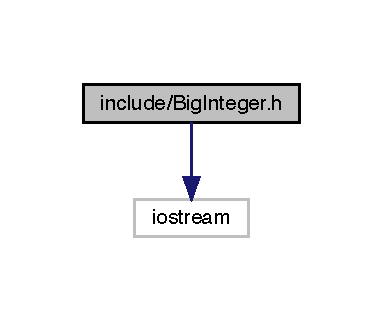
\includegraphics[width=184pt]{_big_integer_8h__incl}
\end{center}
\end{figure}
This graph shows which files directly or indirectly include this file\+:\nopagebreak
\begin{figure}[H]
\begin{center}
\leavevmode
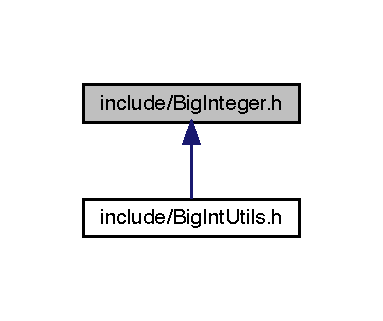
\includegraphics[width=184pt]{_big_integer_8h__dep__incl}
\end{center}
\end{figure}
\subsection*{Classes}
\begin{DoxyCompactItemize}
\item 
class \textbf{ Big\+Integer}
\end{DoxyCompactItemize}


\subsection{Detailed Description}
This project is designed to add a larger integer type to C++. 

\begin{DoxyAuthor}{Author}
Jacob Howell 
\end{DoxyAuthor}
\begin{DoxyDate}{Date}
06/04/2017 
\end{DoxyDate}
\begin{DoxyVersion}{Version}
1.\+0
\end{DoxyVersion}
\subsection{D\+E\+S\+C\+R\+I\+P\+T\+I\+ON}\label{namespacestd_DESCRIPTION}
This program adds a new Integer type for c++ programs. It allows for the use of a much larger Integer value and manipulate it. 
%--- End generated contents ---

% Index
\backmatter
\newpage
\phantomsection
\clearemptydoublepage
\addcontentsline{toc}{chapter}{Index}
\printindex

\end{document}
